%! Suppress = Ellipsis
\chapter[Graphical User Interfaces]{Getting Started with Graphical User Interfaces}\label{ch:starting-gui}

\section{Introduction}\label{sec:gui-introduction}
Building User Interfaces may seem more complicated than what it is. Once you get the fundamentals, you can see that it is possible to put something together very quickly, especially if we already have some code to which to relate. In the previous chapter, we saw that we can control an experiment from the command line. It is possible to ask ourselves why going through the trouble of a user interface. In some cases, it can be very not only handy to control the parameters of an experiment and to monitor the output in a window especially designed, but it can become necessary to monitor the progress in real-time to make decisions while the experiment runs.

There are several options for building GUIs with Python. And in the community, there is no clear consensus on what is the best path to follow. For scientific applications, however, the only library which is powerful enough to achieve what we want to achieve is called \textbf{Qt}. Qt was developed as an application framework that allows developers to build apps that look native in different systems without changes to the code. Qt itself is a Finnish company with a long trajectory. It was part of Nokia for a while, and now they are publicly traded in the Helsinki exchange. It means that Qt is going to be around for a long time.

In this chapter, we are going to give the first steps for building a user interface using Qt, and the Python wrapper called \emph{PyQt}, that we installed in Chapter~\ref{ch:setting-up}. At Python, for the Lab, we have traditionally adopted PyQt, but in the past years, Qt itself took over the project called PySide, which is another wrapper for Qt. They are licensed under different open-source terms, and both are excellent. However, the structure of the PySide2 package is different from the PyQt package, and, for consistency, we keep using PyQt.

\checkInfo{Qt, PyQt, and PySide licensing}{If you are planning to release commercial software, or if you are packaging Qt, PyQt or PySide2 into your application, you should explore the different licensing options available.}


\section{Creating a Simple Window and Buttons}\label{sec:simple-window-andbuttons}
Now it is finally time to start using the empty folder from the M-\textbf{V}-C design pattern: the \textbf{View}. We start by learning how to create simple windows directly with Qt and proceed to a fully-featured user interface for our experiment. We start just with scripts, and we slowly grow in complexity.

The best way to get started with Qt is with a quick example. We can create a new file, \textbf{simple\_window.py} in the \emph{Examples} folder, with this code:

\begin{minted}{python}
    from PyQt5.QtWidgets import QApplication, QMainWindow

    app = QApplication([])
    win = QMainWindow()
    win.show()
    app.exec()
\end{minted}

We will come back to the code above over and over again. In the beginning, it is hard to remember, but once we do it often enough, it sticks. After importing, we create a \py{QApplication}, a \py{QMainWindow}, we show it, and we run the app. This code should produce a very simple window that looks like the image below:

\begin{center}
    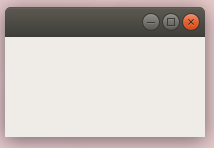
\includegraphics[width=.3\textwidth]{images/Chapter_08/01_simple_window.png}
\end{center}

The style matches the operating system where it runs. It is a simple, empty window. However, we can already start understanding how Qt works. A user interface is a program that keeps running in a loop. When we click and drag to resize a window, for example, there is always a program responsible for knowing how to do it. In Qt, this never-ending loop is the \py{QApplication}. Whatever window we want to create needs to belong to an application, and that is why the first thing we did was defining \py{app}.

In the following line, we define a new object, called \py{win}, which is a \py{QMainWindow}. As the name suggests, the main windows are the core of the user interface. From the main window, we can open dialogs, other windows, but the main window is central to our program. After creating it, we show it. The last line is where the application loop starts. The \py{app.exec()} command is blocking. Therefore nothing that comes after is executed until we finish with the user interface.

\questionInfo{Exercise}{To understand a bit better what is going on with the user interface, you are encouraged to try different things. For example, what happens if you don't show the window or add a few print statements to see when they get executed. You can also try to define the window before the application.}

Having an empty window is not particularly useful, so we can start adding elements to it. First, we add a title to the window, like this:

\begin{minted}{python}
    win.setWindowTitle('My First Window')
\end{minted}

Very slowly, our program starts taking shape and looking more professional. We can also add an interactive element, such as a button. We can define one like this:

\begin{minted}{python}
    from PyQt5.QtWidgets import QApplication, QMainWindow, QPushButton

    app = QApplication([])
    win = QMainWindow()
    win.setWindowTitle('My First Window')
    button = QPushButton('Press Me', win)
    win.show()
    app.exec()
\end{minted}

Which will produce a small window, like this:

\begin{center}
    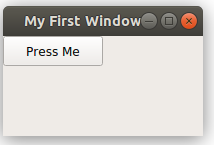
\includegraphics[width=.3\textwidth]{images/Chapter_08/02_simple_window_and_button.png}
\end{center}

Notice that when we defined the button, we added a second argument, \py{win}. Qt has a hierarchical structure, where each element is called a \emph{widget}. We have imported three widgets so far: the application, the window, and the button. All widgets live inside the application loop, but we have to establish the relationship between them. By passing the window as the second argument, we are explicitly saying that the button belongs to the window.

\questionInfo{Exercise}{Remove the \py{win} from the definition of the button, and see what happens}
\questionInfo{Exercise}{Alter the order and make the button the parent of the main window, does this work?}

A big part of working with Qt is finding out how to relate different widgets to each other, how to position them. \py{QMainWindows} are special because they must hold widgets within them. That is why they specify a method to determine which Widget is the most important for the window, or in Qt jargon, which Widget is the central Widget. We can explicitly declare it:

\begin{minted}{python}
    button = QPushButton('Press Me')
    win.setCentralWidget(button)
\end{minted}

We removed the \py{win} from the declaration of the button, but if it's there it doesn't change the behavior. The window now looks somewhat different:

\begin{center}
    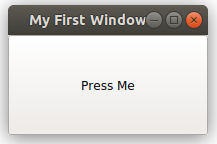
\includegraphics[width=.3\textwidth]{images/Chapter_08/03_simple_window_and_central_widget.png}
\end{center}

You can try resizing the window, and you see that the button scales. By declaring the button as the central Widget of the window, we made the relationship even stronger. The last possibility which is worth mentioning before moving forward is that we can also show the button independently from the window, like this:

\begin{minted}{python}
    win.setWindowTitle('My First Window')
    button = QPushButton('Press Me')
    win.show()
    button.show()
\end{minted}

In this case, the window and the button are two independent components, like we show in the image below. For the program to finish, we must close both the button and the window.

\begin{center}
    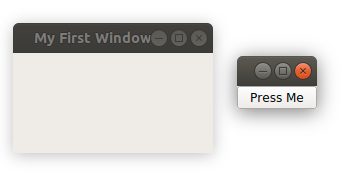
\includegraphics[width=.3\textwidth]{images/Chapter_08/04_window_button_separated.png}
\end{center}

Qt offers a great deal of flexibility, which doesn't mean we need actually to use it. Having buttons floating around the screen does not sound like a good idea, but it is a possibility in case we ever need it.

Now that we have a button on a window, we are craving to do something with it.


\section{Using Signals and Slots}\label{sec:signals-slots}
Qt offers a programming pattern known as \emph{Signals} and \emph{Slots}. The core idea is that different actions on a user interface trigger a signal. For example, moving the mouse over an element triggers a signal. This signal is then caught by \emph{slots}, which do something with the information provided. When we move the mouse over a button (this is also knowns as hovering), its background changes color. It is a clear example of the signal/slot paradigm.

Every Widget that we can place on screen has a myriad of signals. From interactions with the mouse to changes in shape or size triggered by reshaping the window, to time-based signals. It does not mean we need to know them all, nor that we use them all. But once we understand the pattern, we know where to go and find what we are after. The button has one signal called, very eloquently, \py{clicked}. To use it, we must define a function that can be called every time the signal fires. This function is the \emph{slot}. We can expand our example code like this:

%! Suppress = Ellipsis
\begin{minted}{python}
def button_clicked():
    print('Button Clicked')

[...]
button = QPushButton('Press Me')
button.clicked.connect(button_clicked)
win.setCentralWidget(button)
\end{minted}

We can see that every time we click the button, the program prints a message to the screen. It is very important to note that we used \py{button_clicked} and not \py{button_clicked()}. It is the same that we discussed in Section~\ref{subsec:multithreading} when discussing multithreading. We must use the function itself as a slot, and not the outcome of the function.

\subsection{Starting a scan}\label{subsec:start-scan-gui}
With what we have done so far, triggering a scan from the user interface becomes almost trivial. For the time being, we can keep working on the \emph{Examples} folder, but this time let's create a new file called \textbf{start\_gui.py}. We only need that when we press the button, a scan starts. We need to mix what we already have in \textbf{run\_experiment.py} with what we have done above. It can look like this:

\begin{minted}{python}
    from PyQt5.QtWidgets import QApplication, QMainWindow, QPushButton

    from PythonForTheLab.Model.experiment import Experiment

    experiment = Experiment('experiment.yml')
    experiment.load_config()
    experiment.load_daq()

    app = QApplication([])
    win = QMainWindow()
    win.setWindowTitle('My First Window')
    button = QPushButton('Start Scan')

    button.clicked.connect(experiment.do_scan)

    win.setCentralWidget(button)
    win.show()
    app.exec()

    experiment.finalize()
\end{minted}

The code above is a merge between what we did in the previous chapter and this one. We define the experiment as always, and the window and button as we have just learned. However, the line that does all the magic is this one:

\begin{minted}{python}
    button.clicked.connect(experiment.do_scan)
\end{minted}

We can try the program. When we click the button, a scan starts. However, there is something else happening. The window freezes, we are not able to reshape it, close it. In some cases, especially on Windows, the program crashes, and we get a message saying whether we want to report the issue.

\questionInfo{Exercise}{Can you guess why the window freezes?}

When we described the flow of a Qt program, we talked about a loop taking care of the interactions within the program. However, if we trigger a scan using \py{do_scan}, we are going to block that loop. Both Qt and Python are single-threaded applications by default, and when one blocks, the other blocks as well. And by talking about single-threaded applications, we gave a hint to how this can be solved.

At the end of the last chapter, we developed a different method called \py{start_scan} that creates a separate thread to hold the scanning, effectively releasing the main thread to do other tasks. We can change just one line of code and achieve a very different behavior:

\begin{minted}{python}
    button.clicked.connect(experiment.start_scan)
\end{minted}

We have developed a somewhat functional program. We have a window with a button from which we can control our experiment. It is already quite an excellent achievement. We also got some extra features out of the box, such as preventing the user from triggering two scans at the same time.

Sometimes, the easiness of developing this kind of solution misguides the readers. It was so easy to achieve what we achieved so far because we spent a lot of time and effort developing a proper \emph{experiment class}. The threading, the checks to prevent two scans, and some extra things that keep appearing in this and next chapter are thanks to a well-designed model.


\section{Extending the Main Window}\label{sec:extending-main-window}
We have seen how to get started by creating the main window and adding a button to it. However, we can also start seeing that if we try to add more elements, the code is going to become more and more convoluted. It would be a nice addition if the window we design here could be used for different purposes as well. As we have already seen many times, a good idea when we want to make blocks of code reusable is to convert them into classes. Qt is ideally suited for this because every Widget they provide is an object with a special inheritance tree.

In the folder \emph{View} we can create a file called \textbf{main\_window.py}, and we can add the following code:

\begin{minted}{python}
    from PyQt5.QtWidgets import QMainWindow


    class MainWindow(QMainWindow):
        def __init__(self):
            super().__init__()
            self.setWindowTitle('My First Window')
\end{minted}

Before discussing what we have done, we can quickly go back to \textbf{start\_gui.py} and change the following two lines of code:

\begin{minted}{python}
    win = QMainWindow()
    win.setWindowTitle('My First Window')
\end{minted}

with this one:

\begin{minted}{python}
    win = MainWindow()
\end{minted}

We should also remember to change the imports at the top of the file by these:

\begin{minted}{python}
    from PyQt5.QtWidgets import QApplication
    from PythonForTheLab.View.main_window import MainWindow
\end{minted}

If we run the code, we see that it behaves as it was behaving previously. In our code, we create a new class called \py{MainWindow}, which in turn inherits from \py{QMainWindow}. It is always important to call \py{super()} because that runs the init method from the QMainWindow itself, setting up all the parameters, signals, properties that we need to generate a window. There is, however, a difference with a plan \py{QMainWindow}, we specify its title. Effectively, we have now extended the pure \py{QMainWindow} class to include a title by default.

\checkInfo{Naming conventions}{It is a personal preference when I start developing a program that has only one main window to name it \py{MainWindow}, removing the preceding \py{Q}. It can lead to mistakes if we overlook the small difference in both names. Depending on taste, an alternative is to call the windows by what they are supposed to do, such as \py{ScanWindow}. It depends on the reader's preferences.}

We can add the button, and the slot, like this:

\begin{minted}{python}
from PyQt5.QtWidgets import QMainWindow, QPushButton


class MainWindow(QMainWindow):
    def __init__(self, parent=None):
        super().__init__(parent=parent)
        self.setWindowTitle('My First Window')
        self.button = QPushButton('Press Me')
        self.setCentralWidget(self.button)

        self.button.clicked.connect(self.button_clicked)

    def button_clicked(self):
        print('Button Clicked')
\end{minted}

We can test this code again and see that we have recovered what we had before. Every time we press on the button, a message appears on the screen. We can also go one step further and start thinking about how to work with the experiment itself. The window is not aware of any experiments, but we would like to be able to trigger a scan if we press the button. Therefore, the experiment has to come from outside of the class and be stored within.

We have already done something like this. When we developed the driver in Section~\ref{sec:going-higher-level}, we could send the port number to the class through the \py{__init__} method. We did the same for the device model in Section~\ref{sec:device-model}, and for the experiment model in Section~\ref{sec:skeleton-experiment-model}. In all those cases, we were using simple strings, but we are not limited to them. Arguments of methods, or any function for the matter, can be complex objects as well.

We can adapt the \py{MainWindow} to accept an experiment as argument, store it as an attribute and use it when we need to. The code would look like this:

\begin{minted}{python}
    [...]
    class MainWindow(QMainWindow):
        def __init__(self, experiment=None):
            super().__init__()
            self.experiment = experiment

            [...]
        def button_clicked(self):
            self.experiment.start_scan()
            print('Scan Started')
\end{minted}

The changes to the code were minimal but significant. We have included \py{experiment=None} in the init. We have provided a default value for the experiment because this allows us to run the program even if we have no experiment defined. It is useful if we want to test how the window looks like quickly. However, as soon as we press the button, the program crashes. We have to update the \textbf{start\_gui.py} script to accommodate for the changes:

\begin{minted}{python}
experiment = Experiment('experiment.yml')
experiment.load_config()
experiment.load_daq()

app = QApplication([])
window = MainWindow(experiment)
window.show()
app.exec()

experiment.finalize()
\end{minted}

We pass \py{experiment} directly to the window, and it takes care of the rest. We can now safely trigger a scan from the user interface. What is important to note is that once we reach this step, all the rest happens directly on the view. The script that we use to open the window stays unaltered. Even in much more complex programs, we use the same pattern\footnote{See, for example, how PyNTA starts its user interface: https://bit.ly/WindowExperiment}.

\section{Adding Layouts}\label{sec:adding-layouts}
So far, our window holds only one button, and we set that button to be the central Widget of the window. This makes it virtually impossible to add any other button or object. Therefore, it is time to start sophisticating our user interface\footnote{In this chapter we decided to go lower level, programming every feature, but in the next chapter we will see how to do it with the QtDesigner software, which will speed up the process}. The basic building blocks in Qt are \py{QWidgets}, and Qt allows us to place widgets inside of widgets at our will. We also know that Main Windows require a central widget. Therefore, we can create a widget that holds two buttons: start and stop, and that Widget is the central Widget of the window. We use this opportunity to clean up the names we have used, to make them more descriptive as well, it is important to pay attention to all the changes made:

\begin{minted}{python}
from PyQt5.QtWidgets import QMainWindow, QPushButton, QWidget


class MainWindow(QMainWindow):
    def __init__(self, experiment=None):
        super().__init__()
        self.experiment = experiment
        self.setWindowTitle('Scan Window')

        self.button_widgets = QWidget()
        self.start_button = QPushButton('Start', self.button_widgets)
        self.stop_button = QPushButton('Stop', self.button_widgets)

        self.setCentralWidget(self.button_widgets)

        self.start_button.clicked.connect(self.start_scan)

    def start_scan(self):
        self.experiment.start_scan()
        print('Scan Started')
\end{minted}

If we run the program again, we will see a Window like the one below:

\begin{center}
    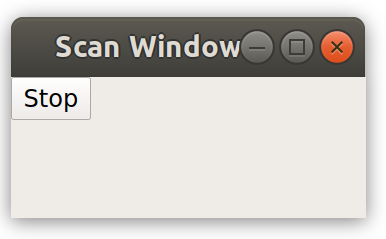
\includegraphics[width=.3\textwidth]{images/Chapter_08/05_window_without_layout.png}
\end{center}

The stop button is visible, but not the start button. It happens because Qt has no way of knowing where we want to add the buttons and place them in the same position. The one that gets added later is on top.

\questionInfo{Exercise}{Change the order in which we define the buttons and see that one or the other gets on top. If the button that is below has a much longer text, you can see it beneath the top one.}

We could specify explicit coordinates for the positions of the buttons, but there is a much simpler approach using layouts. In Qt, there are 4 basic layout types: Horizontal, Vertical, Grid, and Form. With the first two, each time we add a widget, it is added either below or to the right. With the grid layout, we can control the position, width, and height based on a grid we define. The form defines two columns, ideally to hold some labels and inputs. We see more about layouts in the following chapter. For the time being, if we want to add two buttons, we can choose a horizontal layout. The code of the \py{MainWindow} takes a few extra lines to set everything up properly:

\begin{minted}{python}
from PyQt5.QtWidgets import QHBoxLayout
[...]
self.button_widgets = QWidget()
self.start_button = QPushButton('Start')
self.stop_button = QPushButton('Stop')
layout = QHBoxLayout(self.button_widgets)
layout.addWidget(self.start_button)
layout.addWidget(self.stop_button)

self.setCentralWidget(self.button_widgets)
\end{minted}

In Qt, the horizontal layout is called \py{QHBoxLayout}, and we apply it to the \py{buttons_widget}. Then, we add the start and stop to the layout, instead of directly to the widget. This window will look much better:

\begin{center}
    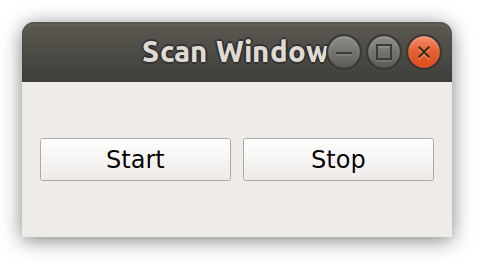
\includegraphics[width=.3\textwidth]{images/Chapter_08/06_window_with_layout.png}
\end{center}

If we resize it, we see that the buttons take the entire width, and they are always centered. It is already a good improvement compared to the simple window with which we started. Before we finish this section, these two exercises are a good way of practicing the skills acquired so far:

\questionInfo{Exercise}{Change \py{QHBoxLayout} by \py{QVBoxLayout} to see the buttons stacked vertically.}

\questionInfo{Exercise}{Connect the stop button to a method that stops the scan}

\section{Plotting Data}\label{sec:plotting-data}
We finish this section by adding a plot of the data in real-time. We already did something similar in Section~\ref{sec:basic-plotting}. Parts of the code are very similar. Our window slowly starts getting more complex, with more elements. So far, we have two buttons stacked horizontally, but we would like to show the plot beneath the buttons, not next to them. One of the most natural solutions is to start stacking widgets, instead of making the \py{buttons_widget} the central Widget, we can make another one that contains the buttons and the plot.

\begin{minted}{python}
import pyqtgraph as pg
from PyQt5.QtWidgets import (QMainWindow,
                             QPushButton,
                             QWidget,
                             QHBoxLayout,
                             QVBoxLayout, )

class MainWindow(QMainWindow):
    def __init__(self, experiment=None):
        super().__init__()
        self.experiment = experiment
        self.setWindowTitle('Scan Window')

        self.central_widget = QWidget()
        self.button_widgets = QWidget()
        self.start_button = QPushButton('Start')
        self.stop_button = QPushButton('Stop')
        self.plot_widget = pg.PlotWidget(title="Plotting I vs V")
        self.plot = self.plot_widget.plot([0], [0])

        layout = QHBoxLayout(self.button_widgets)
        layout.addWidget(self.start_button)
        layout.addWidget(self.stop_button)

        central_layout = QVBoxLayout(self.central_widget)
        central_layout.addWidget(self.button_widgets)
        central_layout.addWidget(self.plot_widget)

        self.setCentralWidget(self.central_widget)
\end{minted}

Some remarks about the code before we run it. We are using \py{()} for the import because it makes it easier to stack the modules instead of having a very long line that becomes hard to read. In the window, we define three widgets now, \py{central_widget}, \py{button_widgets}, and \py{plot_widget}. The plot widget is very similar to what we did in the previous chapter. The only difference is that we store the Widget itself and the plot separately, and we explain why later. We didn't touch the buttons, but instead of adding them as the central Widget, we add them to a higher-order widget. By stacking the buttons horizontally between themselves, but vertically to the plot, we get a window that looks like this:

\begin{center}
    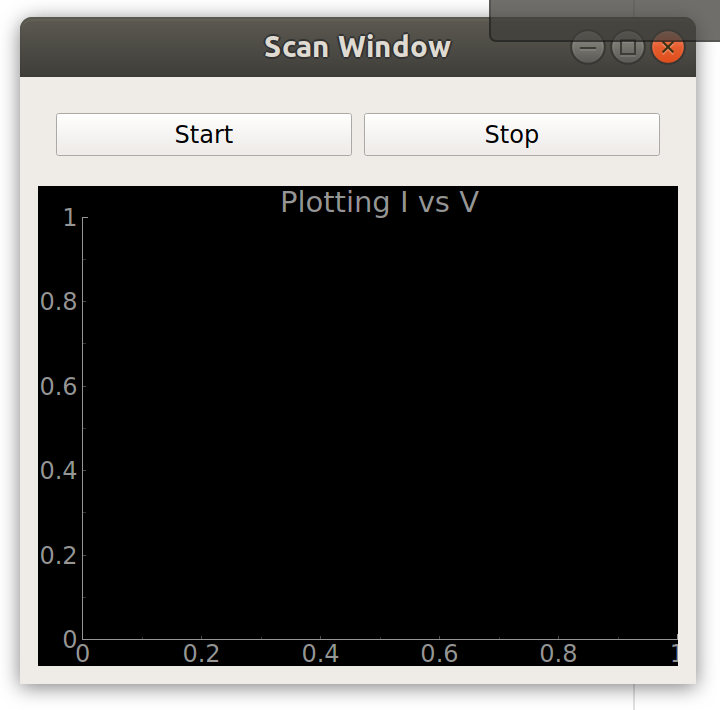
\includegraphics[width=.4\textwidth]{images/Chapter_08/07_window_empty_plot.png}
\end{center}

We are halfway through with what we wanted. If we resize the window, the plot changes, taking all the space available, even if we expand the window vertically, there is no gray area around the buttons. How the surrounding elements control the shape of a widget is one of the properties that can be specified.

\tipsInfo{Qt options}{We make several remarks about possibilities with Qt that we don't explore further. We just want to point out that every single thing that happens on a user interface was decided, and can be changed. Not only the aspect, such as colors but also how different elements relate to each other and change shapes when the container window changes.}

To plot the data we acquire, we just need to update the plot periodically. Qt offers a special object called \py{QTimer} that also specifies signals. With timers, we can trigger periodic actions without interrupting the rest of the program. We also need to develop a method that can update the plot. The Main Window code looks like this:

\begin{minted}{python}
    from PyQt5.QtCore import QTimer
    [...]

    class MainWindow(QMainWindow):
        def __init__(self, experiment=None):
            [...]
            self.timer = QTimer()
            self.timer.timeout.connect(self.update_plot)
            self.timer.start(50)

        def update_plot(self):
            self.plot.setData(self.experiment.scan_range, self.experiment.scan_data)
\end{minted}

The timer is relatively easy to understand. It is an object that triggers a signal, \py{timeout} periodically. We connect that signal to the method \py{update_plot}. When we start the timer, we need to specify the time interval in milliseconds, therefore $50\,\textrm{ms}$ means a refresh rate of $20\,\textrm{Hz}$. The \py{update_plot} method is different from what we did in the previous chapter. Instead of using \py{plot}, we are using \py{setData}. There are two reasons for it. First, if we use \py{plot()}, we create a new plot on top of the existing one. We wouldn't be refreshing the data but drawing on top of it. After a while, especially if the parameters or results change, we would see several lines overlapping. The second reason is speed. \py{plot()} is a relatively slow method because several things need to be set up, such as the axes, labels, ticks. By using \py{setData} PyQtGraph automatically reuses the elements available.

However, if we try to run the code, we will get a problem:

\begin{minted}{bash}
    AttributeError: 'Experiment' object has no attribute 'scan_range'
\end{minted}

\questionInfo{Exercise}{Find out why are we getting this error even though we didn't find it when running a more straightforward script in the previous chapter}

When the window starts, we automatically start the timer, which, in turn, tries to update the plot. However, the experiment class does not have any \py{scan_range} nor \py{scan_data} until the experiment starts running. A bypass to the problem would be to start the timer after we have started the scan, but this is very unreliable. Best-practices in Python indicate that we should always define attributes in classes in the \py{__init__} method. It means that as soon as we create the object, the attributes exist, even if with place-holder values.

When we developed the \emph{Experiment class}, we completely neglected this practice. We added \py{self.} whenever we needed to have data available through the class and also from outside of it. We leave the definition of most of the attributes to the reader, but we show how to solve the problem with the scan. Going back to the experiment model, we need to add the following:

\begin{minted}{python}
    class Experiment:
        def __init__(self, config_file):
            [...]
            self.scan_range = np.array([0]) * ur('V')
            self.scan_data = np.array([0])  * ur('V')
\end{minted}

We decided to define both attributes as numpy arrays holding only one value: $0\,\textrm{V}$. If we try to plot these results, we get a single point at the origin. It may raise other questions, such as whether it is better to have a $0$ or a \py{None} value, because $0\,\textrm{V}$ could be a valid measured value. It is left to the sensitivity of the reader to judge what is best in their specific case. For our purposes, this is enough to get the window running and showing a plot of the data in real-time once the scan starts.

\questionInfo{Exercise}{Every attribute in any class should be defined in the init of that class. Go through all the models, and see whether there are attributes used but not defined at instantiation.}

\subsection{Increasing the refresh rate and number of data points}\label{subsec:refresh-rate-and-number-of-data-points}
When we follow the strategy of using a timer for refreshing the plot, we can be tempted to increase the refresh rate to make the animations more appealing, but we have to be careful with this. On the one hand, if we are generating data at, let's say, $1\,\textrm{Hz}$, doesn't matter how fast we refresh the plot, it won't change faster than once per second.

Let's assume we are acquiring data much faster than once per second, perhaps at hundreds or thousands of new points per second. We have to consider how fast the screen of the computer can redraw the elements on it. Most screens work at $30\,\textrm{Hz}$, some may go to $60\,\textrm{Hz}$. Therefore, if we try to update the plot faster than that, we just waste computer power on something that the screen never can show us.

There is one additional limitation that is our own eyes. We can't process images faster than at 30fps. Already at $50\,\textrm{Hz}$, we don't see the lights in our room blinking. If we are not interested in video quality for the update of our plots, we can safely go down to $20\,\textrm{Hz}$, and the images still look fluid.

\questionInfo{Exercise}{Instead of plotting data from the device, you can update the plot with points that oscillate in time and see up to which point the refresh rate affects the quality of what you are showing.}

There is one more thing to consider beyond the refresh rate, which is the number of points we are plotting. Most screens have a few thousand pixels in each direction. A very common resolution is $1920\times1440\,\textrm{pixels}$. If we acquire $10000$ data points and try to show them on the screen, they have to be reduced almost 5 times to fit the number of pixels available on the screen. In this reduction process, we can lose many details. If we use downsampling, for example, and we are looking for a narrow peak, the chances of it appearing on the image can be very little.

We have to be aware of the number of data pixels that we try to show not only on user interfaces but also when we are preparing plots for printing or inserting into a PDF. The number of dots a printer can generate is normally specified as dots per inch, or dpi. Even at $600\,\textrm{dpi}$, an image with a width of $8\,\textrm{cm}$ (standard 1-column figure on a paper) will have under 2000 dots in its horizontal direction. And, of course, a reader behind a computer screen is limited to its pixels.

\section{Conclusions}\label{sec:basic-gui-conclusions}
In this chapter, we have started building a user interface for the experiment. We explored how to get started with Qt, PyQt, how to use buttons to trigger actions using signals and slots. We also saw how to connect a basic user interface to the experiment model. It showed us the advantages of having an experiment that already runs measurements in its threads.

We also saw how to extend the basic building blocks of Qt, such as QMainWindow, by subclassing it and adding the elements we needed. We saw how to build widgets with more widgets inside, how to lay them out on more complex patterns. Finally, we added simple plotting capabilities to the window, refreshing whatever data the experiment is acquiring in real-time.

This chapter typically generates much satisfaction for people who are developing user interfaces for the first time. On the other hand, we have done much work, and we got a window that does not look nearly as nice as the windows with which we are familiar from other programs. On the one hand, this helps us understand how much effort is behind every window we see. On the other, it pushes us to go one step further.

In the next chapter, we start seeing how to improve the design of our User Interfaces by using a program called Qt Designer.
